
\lstset{basicstyle=\ttfamily,
  showstringspaces=false,
  commentstyle=\color{red},
  keywordstyle=\color{blue}
}

\section{Wdrożenie i instalacja systemu}

% 192.168.1.126:3000
 
Do uruchomienia serwera webowego zastosowano mini-komputer Raspberry PI z zainstalowanym systemem operacyjnym Raspberry Pi OS, który
z kolei bazuje na Debian'ie. Sam program serwera został zaś zdockeryzowany w celu lepszej współpracy z systemem oraz zapewnienia większej przenośności
aplikacji. Zrezygnowano z lokalnie hostowanej bazy danych na rzecz zewnętrznego serwera MongoDB Atlas \cite{atlas}.

\subsection{Raspberry PI}
W tym projekcie wykorzystano Raspberry Pi model B (4gb RAM, Quad core Cortex-A72 (ARM v8) 64-bit, 16gb pamięci dyskowej) \cite{raspberry}.
Podstawowym czynnikiem, który przeważył o wybraniu tej platformy jako hosta serwera aplikacji webowej była dostępność oraz minimalizacja kosztów eksploatacji.
Hostowanie dynamicznej aplikacji webowej na należącym do nas komputerze pozwala nam w pełni wykorzystać jego możliwości - jesteśmy ograniczeni tylko
pojemnością dysku, ilością pamięci RAM, siłą procesora itd. po kosztach zużytego przez RPI prądu. W przypadku zewnętrznych hostingów mamy do czynienia z
planami, które różnią się ceną oraz dostępnymi zasobami, nie mówiąc już o możliwości zmiany regulaminu bądź planu przez dostawcę.

Takie rozwiązanie ma oczywiście też swoje wady, między innymi ręczna konfiguracja czy 100\% odpowiedzialność właściciela za jakiekolwiek błędy.

\subsection{Dokeryzacja}
W celu zapewnienia poprawnego działania oraz większej przenośności serwera zdecydowano się na konteneryzację aplikacji. Na początku kroku wdrażania podjęto próby 
nad uruchomieniem serwera jako 'zwykły' proces, natomiast rozwiązanie to wielokrotnie wydłużało proces instalacji jak i wymagało instalacji lokalnej wszystkich
paczek wykorzystywanych przez serwer. Zmniejszało to już i tak niską pojemność dysku oraz wprowadzało pewne konflikty między bibliotekami Node a systemem, których
nie udało się naprawić.

Dockeryzacja eliminuje wszystkie powyższe problemy, dodatkowo zapewniając przenośność serwera na inny system (komputer), który pracuje w tej samej architekturze co RPI.

Proces ten polega na tworzeniu 'obrazów' - swoistych szkiców, rusztowań aplikacji. Komputer wyposażony w silnik Dockera oraz posiadający obraz aplikacji jest w stanie 
utworzyć 'kontener' na podstawie tego obrazu. Kontener jest procesem bądź aplikacją uruchomioną wewnątrz środowiska Dockera, który z kolei może zostać uzewnętrzniony do 
hostującego komputera bądź sieci za pomocą przekierowywania portów. Pojedynczy obraz może zostać wykorzystany do stworzenia dowolnej liczby kontenerów, które
można zatrzymywać, restartować lub nawet usuwać.

Sercem procesu dokeryzacji jest plik 'Dockerfile', który zawiera warstwy (reguły, komendy), na podstawie których tworzony jest obraz. Na potrzeby tego projektu zastosowano
dwustopniowy proces budowania. Pierwszy stopień tworzy środowisko z zainstalowanym Node'm, kopiuje do niego pliki źródłowe aplikacji oraz ją buduje. Drugi stopień tworzy osobne
ale identyczne środowisko do tego ze stopnia pierwszego, ale kopiuje do niego tylko pliki niezbędne do uruchomienia aplikacji, które pochodzą ze stopnia pierwszego. 
Takie podejście polegające na zbudowaniu aplikacji w jednym 'miejscu', a następnie przeniesieniu produktu do drugiego zmniejsza rozmiar obrazu około 10-krotnie.

\begin{figure}[H]

\centering
\begin{subfigure}{0.4\textwidth}
    \centering
    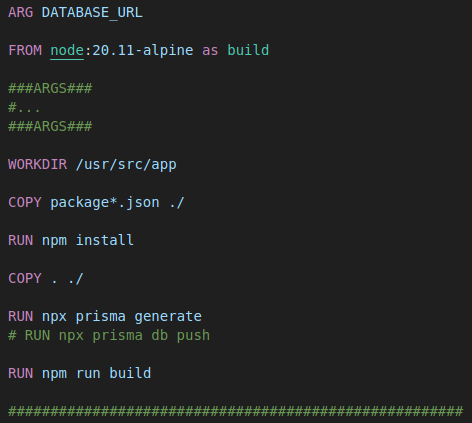
\includegraphics[width=1\linewidth]{zdj/docker_1_cut1.png}
    \caption{Krok 1}
\end{subfigure}
\begin{subfigure}{0.4\textwidth}
    \centering
    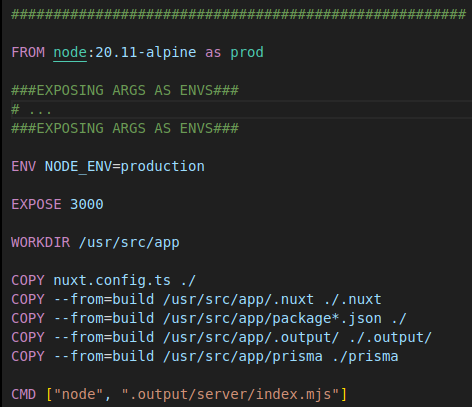
\includegraphics[width=1\linewidth]{zdj/docker_1_cut2.png}
    \caption{Krok 2}
\end{subfigure}
\caption{Plik Dockerfile. Dla estetyki usunięto fragmenty, w których przekazywane są argumenty między krokami}

\end{figure}

Bardzo pomocnym, ale nie niezbędnym narzędziem jest Docker Compose. Jest to osobne narzędzie CLI wykorzystujące plik w formacie YAML. Plik ten zawiera wszystkie informacje
oraz opcje przekazywane przed rozpoczęciem budowania do silnika Docker'a, między innymi: 
\begin{itemize}
    \item architektura procesora systemu docelowego
    \item zmienne środowiskowe, które mają naleźć się w obrazie (klucze API, ustawienia Node, etc.)
    \item ustawienia portów
\end{itemize}

W przypadku nie zastosowania Docker Compose oraz chcąc tworzyć obraz z wszystkimi wymaganymi argumentami, opcjami, itd. należało by każdorazowo wprowadzać je przy wpisywaniu
polecenia w CLI, dla tego Compose jest praktycznie obowiązkowy przy większych projektach.

\begin{figure}[H]
    \centering
    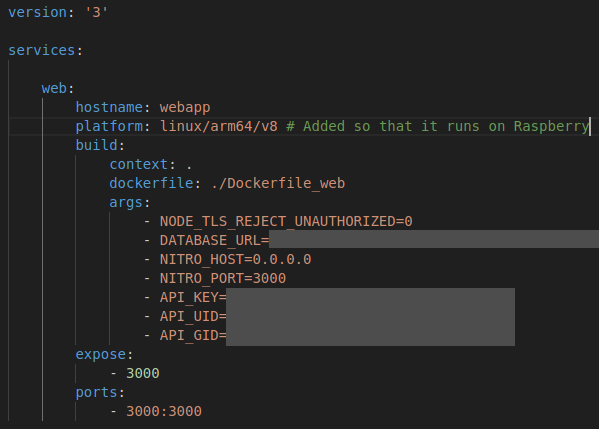
\includegraphics[width=0.7\textwidth]{zdj/compose_1_cenz.png}
    \caption{Plik docker-compose.yaml. Ocenzurowano hasła i klucze API}
\end{figure}

Obraz budujemy komendą
\begin{lstlisting}[language=bash]
    $ docker compose -f docker-compose.yaml build
\end{lstlisting}

Jako, że w komendzie budowania nie zawarliśmy docelowej nazwy pliku, to nazwa obrazu zależy od folderu, w którym Dockerfile się znajduje oraz od nadanej
nazwy serwisu w pliku docker-compose.yaml. W tym przypadku nazwa obrazu to 'webapp-web'. Listę dostępnych obrazów zawsze można sprawdzić za pomocą 

\begin{lstlisting}[language=bash, label={lst:image-ls}]
    $ docker image ls
\end{lstlisting}

Tak zbudowany obraz następnie zamykamy w archiwum, co umożliwia jego przeniesienie na inny system:

\begin{lstlisting}[language=bash]
    $ docker save -o ./webapp_img.tar webapp-web
\end{lstlisting}

\subsection{Uruchomienie na RPI}
W pierwszej kolejności należało zainstalować silnik Docker'a na RPI, co zrobiono za pomocą instrukcji \cite{dockerRPI}. Następnie pobrano zbudowany obraz z komputera,
na którym był budowany na Raspberry Pi. Należy zaznaczyć, że obraz był budowany na innym komputerze, a nie bezpośrednio na RPI ze względu na powolność wykonywania
tej operacji - około 45min.
Aby załadować obraz zapakowany w archiwum tar należy przenieść się do folderu zawierającego archiwum oraz użyć komendy

\begin{lstlisting}[language=bash]
    $ docker load -i webapp_img.tar
\end{lstlisting}

Poprawność wykonania operacji możemy potwierdzić komendą \lstinline|docker image ls| - powinniśmy widzieć nasz obraz w liście.

Jako, że dopuszcza się możliwość przerw w zasilaniu serwera, na przykład poprzez przeniesienie go z sali A do sali B, napisano prosty
skrypt uruchamiający serwer krótki czas po włączeniu RPI:

\begin{lstlisting}[language=bash]
    sleep 30
    sudo docker run -p 3000:3000 -d webapp-web
\end{lstlisting}

\lstinline|sleep 30| ma na celu poczekanie, aż system całkowicie się załaduje. Rozważano obserwacje statusu aktywności silnika Dockera 
jako wskaźnika gotowości systemu, natomiast podjęto decyzję, że to rozwiązanie było by zbyt skomplikowane niż aplikacja tego wymaga.
Druga linijka uruchamia serwer w trybie 'bezgłowym', niegenerującym wyjścia na terminalu oraz uzewnętrznia wewnętrzny port Dockera
do komputera, który ten silnik hostuje. Dzięki temu komputery z sieci lokalnej po wpisaniu adresu RPI oraz portu, na którym działa serwer są 
w stanie korzystać z aplikacji.
 
Skrypt ten zapisano się w dowolnym folderze (tutaj /home/tft/AiRQuality/). Następnie dodano ten skrypt do tabeli Cron wraz z adnotacją, że
ma się wykonywać po każdym starcie systemu. Robi się to za pomocą komendy \lstinline|crontab -e|, co otwiera plik zawierający tzw. 'cron-table'.
Na dole tego pliku dodano się taki oto wpis:

\begin{lstlisting}[language=bash]
    @reboot sh /home/tft/AiRQuality/<nazwa_pliku>
\end{lstlisting}

Plik zapisujemy. Od teraz po każdym starcie systemu będzie wykonany skrypt pod podaną ścieżką.

\subsection{Baza danych} 

\subsubsection{Zakładanie bazy}

Ze względu na problemy instalacji silnika bazy danych (MongoDB) lokalnie na RPI, jedynie około 1,5GB wolnego miejsca na dysku po instalacji 
serwera oraz o wiele wygodniejszą interakcję z bazą danych zdecydowano się na zewnętrzny hosting - MongoDB Atlas \cite{atlas}. Z punktu 
widzenia serwera aplikacji webowej nie zmienia się nic poza adresem bazy danych.

Po założeniu konta w serwisie i zalogowaniu w oknie ukazuje się nam okienko:

\begin{figure}[H]
    \centering
    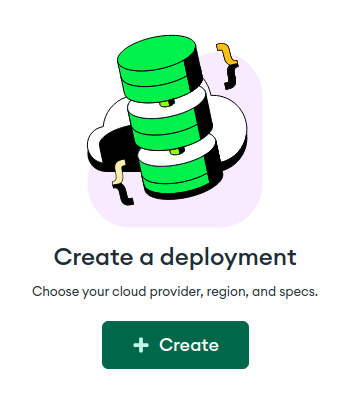
\includegraphics[width=0.5\textwidth]{zdj/atlas_1.png}
    \caption{Twożenie deployment'u}
\end{figure}

Przechodzimy przez ekran tworzenia deployment'u baz danych dostosowując go do naszych potrzeb (rodzaj API, plan płatny lub darmowy, etc.). W 
tym projekcie pozostawiono domyślną nazwe klastra 'Cluster0'. W celu założenia bazy danych projektu należy wybrać opcję 'View Deployment'

\begin{figure}[H]
    \centering
    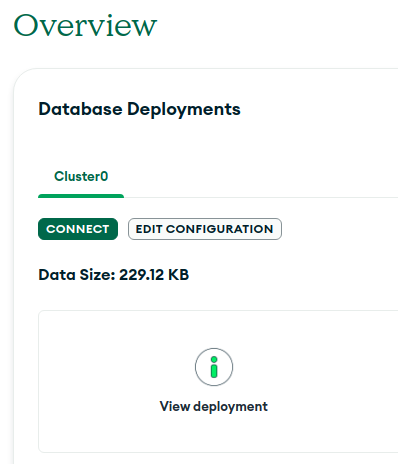
\includegraphics[width=0.5\textwidth]{zdj/atlas_2.png}
    \caption{Wchodzenie w szczegóły deployment'u}
\end{figure}

Następnie przechodzimy do zakładki 'Collections', gdzie tworzymy bazę danych (pojedynczy deployment może mieć wiele baz danych)

\begin{figure}[H]
    \centering
    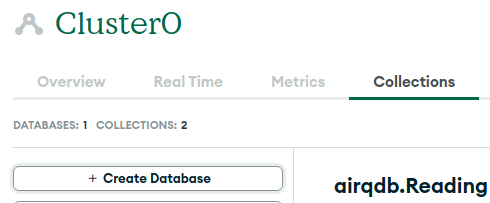
\includegraphics[width=0.5\textwidth]{zdj/atlas_3.png}
    \caption{Tworzenie bazy danych}
\end{figure}

Następnie tworzymy dwie kolekcje, pierwsza z nich będzie reprezentować dostępne w systemie czujniki, druga zaś pozyskane z nich odczyty. Dokładny
kształt bazy jest opisany w rozdziale \ref{ch:baza-danych}.

Aby uzyskać adres bazy danych, z którą aplikacja ma się komunikować przechodzimy do zakładki 'Deployment' widocznej po lewej stronie w menu, a następnie 
w okienku naszego klastra wybieramy opcję 'Connect'. 

\begin{figure}[H]
    \centering
    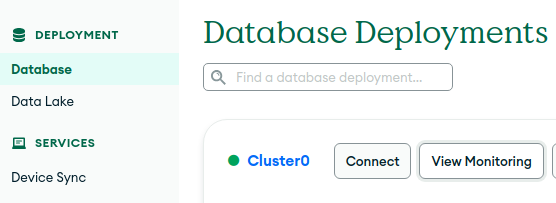
\includegraphics[width=0.5\textwidth]{zdj/atlas_4.png}
    \caption{Odczytywanie szczegółów bazy danych dotyczących podłączenia}
\end{figure}

W wyskakującym okienku wybieramy opcję 'Connect to your application > Drivers'. W następnym kroku 
dobieramy odpowiednie dla nas opcje - wersja MongoDB oraz rodzaj i wersja sterownika. W tym samym oknie ukazuje się nam adres łączący do bazy danych

\begin{figure}[H]
    \centering
    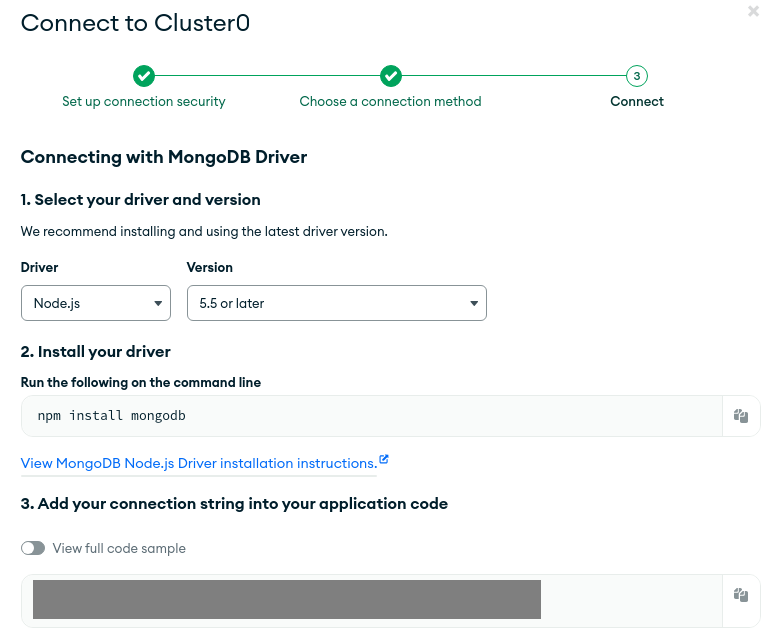
\includegraphics[width=0.5\textwidth]{zdj/atlas_5_cenz.png}
    \caption{Okno szczegółów dot. połączenia. Klucz API ocenzurowano}
\end{figure}

Adres ten udostępniamy naszej aplikacji, w tym wypadku poprzez zmienną środowiskową.

\subsubsection{Obsługa bazy}

\paragraph{Edycja krotki (dokumentu)} \

W trakcie eksploatacji systemu może zajść potrzeba ręcznej modyfikacji którejś z kolekcji, na przykład w wypadku przeniesienia czujnika do innej sali należało by
zmienić przypisaną mu nazwę sali w bazie danych. W tym celu przechodzimy do widoku naszego klastra 'Cluster0', następnie do zakładki 'Collections' i wybieramy 
bazę, a w niej rekordy, które chcemy edytować

\begin{figure}[H]
    \centering
    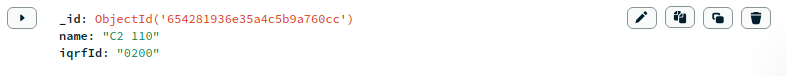
\includegraphics[width=0.7\textwidth]{zdj/atlas_6.png}
    \caption{Przykładowy rekord (dokument) z bazy}
\end{figure}

I wybieramy opcję 'Edit document' (ikona kredki). Operacje usuwania czy kopiowania wykonuje się analogicznie, tylko wybierając inną opcję.

\paragraph{Pobieranie kolekcji} \

Atlas sam w sobie nie udostępnia opcji pobrania zawartości bazy danych lub kolekcji w wygodnym formacie. W tym wypadku 
trzeba posłużyć się narzędziem \lstinline|mongoexport|:

\begin{lstlisting}{language=bash}
    mongoexport --uri \ 
    <adres_klastra>/<nazwa_bazy> \ 
    --collection <nazwa_kolekcji> --out <plik_export>
\end{lstlisting}

Powyższe instrukcje oczywiście przedstawiają jedynie ułamek możliwości systemu, natomiast oceniono je jako opisujące najczęściej występujące problemy. 

\subsection{Dostęp do aplikacji}

Serwer został uruchomiony w sieci domowej SolarLab'u na Politechnice Wrocławskiej. Ze względu na mocno lokalny charakter
nie zarezerwowano nazwy domeny ani nie uzewnętrzniono serwera na Internet. Zamiast tego, każdy komputer znajdujący się w tej samej sieci co serwer RPI 
będzie w stanie uzyskać dostęp do aplikacji po wpisaniu w okno URL adresu \lstinline|192.168.1.126:3000|.

Ustawienie stałego adresu IP w Raspberry Pi dokonujemy poprzez wpisanie do konsoli polecenia \lstinline|hostname -I|. W wyniku otrzymamy m.in. aktualny adres IP urządzenia.
Krok ten pozwala upewnić się, że w następnym kroku nie przypiszemy urządzeniu adresu, który jest już wykorzystywany przez inne urządzenie w sieci.

Następnie klikamy na ikonę WiFi w prawym górnym rogu ekranu RPI. Wybieramy opcję 'Edit connections...'.
Z listy dostępnych sieci wybieramy tą, która nas interesuje. W następnym widoku powinniśmy zobaczyć pustą listę adresów IP. Klikamy opcję 'Add', wpisujemy 
w pierwszą rubrykę adres uzyskany z komendy \lstinline|hostname -I|, w drugą maskę podsieci (tutaj 24-bitowa), w trzecią adres bramy (192.168.1.1).
